\section{Mesures intermédiaires sur le capteur}
\label{chap:mesures}
\subsection{Vérification du corps de chauffe}
Avant toute chose, afin de pouvoir suivre tous les paramètres et le fonctionnement de notre système, une caméra thermique a été utilisée
pour observer le comportement du corps de chauffe

\begin{figure}[H]
    \begin{subfigure}[b]{0.3\textwidth}
        \hspace{-1 cm}
        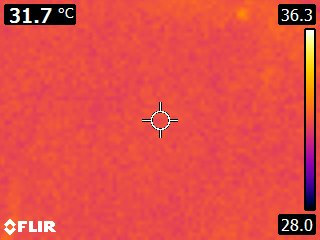
\includegraphics[scale = 0.5]{assets/figures/thermique_sans_chauffe.jpg}
        \caption{Image thermique du capteur - Corps de chauffe éteint}
    \end{subfigure}
    \begin{subfigure}[b]{0.3\textwidth}
        \centering
        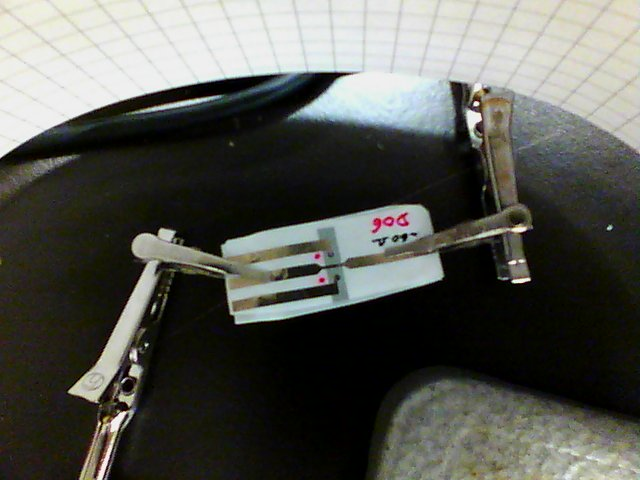
\includegraphics[scale = 0.23]{assets/figures/visuel_avec_chauffe.jpg}
        \caption{Image numérique}
    \end{subfigure}
    \begin{subfigure}[b]{0.4\textwidth}
        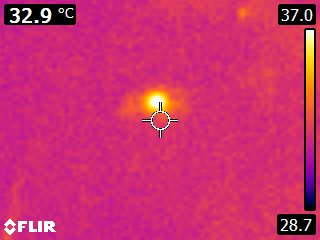
\includegraphics[scale = 0.5]{assets/figures/thermique_avec_chauffe.jpg}
        \caption{Image thermique du capteur - Corps de chauffe allumé}
    \end{subfigure}
    \caption{Résultats de la caméra thermique}
    \label{fig:cameraThermique}
\end{figure}

Il faut savoir que les pistes d'or réfléchissent énormément. Il est donc difficile d'obtenir un résultat parfait. Une première astuce a été de
dessiner au stylo un point noir sur les pistes à mesurer. Ainsi, les problèmes de réflexions seraient amoindris. Malheureusement cette astuce n'a
pas été suffisante. \\

Une autre mesure a alors été faite dans des conditions moins lumineuses (après le coucher du soleil). La figure \ref*{fig:cameraThermique},
montre que le corps de chauffe possède une température avoisinant les 37\textdegree. \\

Un second type de mesure permettant de comprendre chaque partie du \gls{capteur} a été effectuée. Celle-ci concerne la résistance du corps de
chauffe.
\begin{table}[H]
    \begin{center}
        \begin{tabular}{|c|c|c|}
            \hline
            Échantillon n\textdegree & Résistance directe [$\Omega$] & Résistance pointes ressort [$\Omega$] \\
            \hline
            D04                      & 28.28                         & 27.58                                 \\
            \hline
            D06                      & 81.85                         & 72.34                                 \\
            \hline
        \end{tabular}
        \caption{Résistance à travers les pointes ressort}
        \label{tab:resistancePointeRessort}
    \end{center}
\end{table}
Sur le tableau \ref*{tab:resistancePointeRessort}, une différence entre la resistance mesurée directement sur la piste d'or du corps de
chauffe (résistance appelée Résistance directe) et la résistance à travers les pointes ressort est visible. Ceci peut être dû au fait que
les pointes ressort ont également une petite résistance qui vient alors changer la résistance totale du corps de chauffe. Cependant, il faut
également prendre en compte le fait que la résistance change suivant la position de la mesure. En effet, une mesure faite aux extrémités de
la piste d'or sera différente d'une mesure effectuée sur le centre de la piste d'or.

\subsection{Hypothèses concernant l'échantillon défectueux}
Afin de détecter où se situe le problème, les différents paramètres du capteur \gls{capteur} ont été remis en question :
\begin{itemize}
    \item \textbf{Matériau thermoélectrique (ThEl)}\\
          La solution de Tellure de Bismuth est peut-être impure. Une nouvelle solution a été alors refaite.

    \item \textbf{Distance des pistes d'or du capteur au corps de chauffe}\\
          La distance entre le corps de chauffe et les piste d'or peut être importante, car trop proches, les unes des autres, la chaleur du corps
          de chauffe risque de se transmettre aux deux extrémités du capteur. De ce fait, la même température sera mesurable en tout point du
          capteur, engendrant donc aucune différence de température entre la partie droite et la partie gauche du \gls{capteur}, et donc aucune
          tension ne sera mesurable.\\

    \item \textbf{Epaisseur de la membrane} \\
          Plus la membrane est épaisse, plus la couche d'or de court-circuit sera éloignée. Cela permettrait à la source de chaleur d'être concentrée
          à un endroit spécifique. Ceci est important pour des raisons similaires au premier paramètre cité. Un transfert de chaleur faible (voir
          inexistant) entre les deux extrémités du \gls{capteur} est souhaitable (c'est la différence de température qui va engendrer une tension
          mesurable). \\

          Dans le stock de matière de membranes se trouvent les choix suivant :
          \begin{itemize}
              \item GTTP 6-10$\mu$m d'épaisseur
              \item VCTP 6-10$\mu$m d'épaisseur
              \item PI25005 25$\mu$m d'épaisseur
          \end{itemize}
          L'objectif sera alors de faire des capteurs en PI25005 (Kepton) et de les comparer grâce au banc de test aux échantillon en GTTP ou VCTP.
          Ceci permettra de affirmer ou désaffirmer l'hypothèse.\\

    \item \textbf{Diamètre du via}\\
          Lors de l'électrodéposition, un joint en caoutchouc percé au centre d'un diamètre de 0.3mm, 0.5mm ou 1mm (appelé diammètre du via) permet de concentrer
          l'électrodéposition aux endroits souhaités. Cependant, si le diamètre du via est trop faible, l'électrodéposition peut avoir du mal à
          se produire (phénomènes de bulles, électrodéposition non-régulière, etc.)\\

    \item \textbf{Position de la piste de court-circuit}\\
          Afin de s'assurer que le corps de chauffe de transmet pas la chaleur au deux extrémités du capteur, il serait possible de placer la couche
          d'or de court-circuit plus distantes aux électrodépositions
\end{itemize}

\section{Résultats concluants}
Avec une nouvelle solution de Tellure de Bismuth et deux nouvelles électrodépositions sur une membrane de GTTP, de nouvelles mesures ont été
effectuées. Ces mesures nous ont montré que le capteur fonctionnait. En effet, une réponse a été mesurée.
\begin{table}[H]
    \begin{center}
        \begin{tabular}{|c|c|}
            \hline
            Condition du capteur                                   & Tension mesurée à travers l'amplificateur \\
            \hline
            Corps de chauffe désactivé et arrivée d'air désactivée & 5 mV                                      \\
            \hline
            Corps de chauffe activé et arrivée d'air désactivée    & 0 V                                       \\
            \hline
            Corps de chauffe activé et arrivée d'air activée       & 8 mV                                      \\
            \hline
        \end{tabular}
    \end{center}
\end{table}
Malgré le bruit non-négligeable mesuré à travers l'amplificateur, la tension change suivant les conditions du capteur.

\section{Dépandances}
\section{Discussion}